
%
% SECTION: The method
%
\section{The method}
\begin{frame}
    \frametitle{Summary}
    \tableofcontents[currentsection, hideothersubsections]
\end{frame}


\subsection{Management of risk}
\begin{frame}
    \frametitle{A Structured, Iterative and Qualitative method}
    \framesubtitle{}
    \begin{columns}[t]
        \begin{column}{5.5cm}
            \begin{figure}
            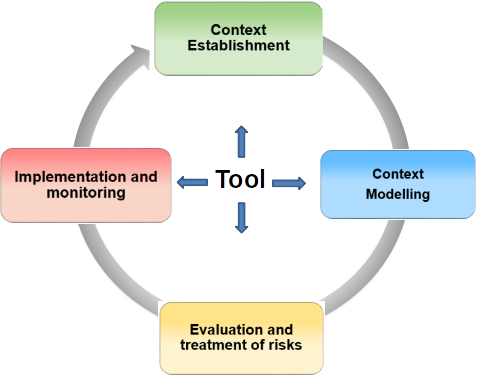
\includegraphics[width=5.5cm]{./images/MONARC-method-1.png}
            \end{figure}
        \end{column}
        \begin{column}{6.5cm}
            \begin{itemize}
                \item Structured: 1, 2, ..., n.
                \item Iterative: \textbf{Plan}, \textbf{Do}, \textbf{Check}, \textbf{Act}
                \item Qualitative: \textbf{Values} / \textbf{Consequence}
                \begin{itemize}
                    \item Impact/Consequence, Threat, Vulnerability;
                    \item \textbf{r}eputation, image;
                    \item \textbf{o}peration;
                    \item \textbf{l}egal;
                    \item \textbf{f}inancial;
                    \item \textbf{p}erson (to the).
                \end{itemize}
            \end{itemize}
        \end{column}
    \end{columns}
\end{frame}

\begin{frame}
    \frametitle{Automated and simplified management}
    \framesubtitle{Method based on \texttt{ISO/IEC 27005}}
    \begin{center}
        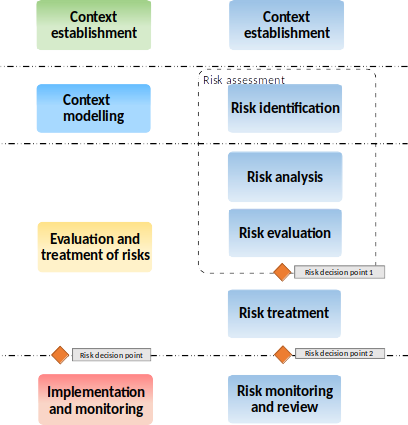
\includegraphics[scale=0.45]{./images/MONARC-method-2-2.png}
    \end{center}
\end{frame}

\begin{frame}
    \frametitle{Automated and simplified management}
    \framesubtitle{Sub-stages provided by the method are also in line with \texttt{ISO/IEC 27005}}
    \begin{center}
        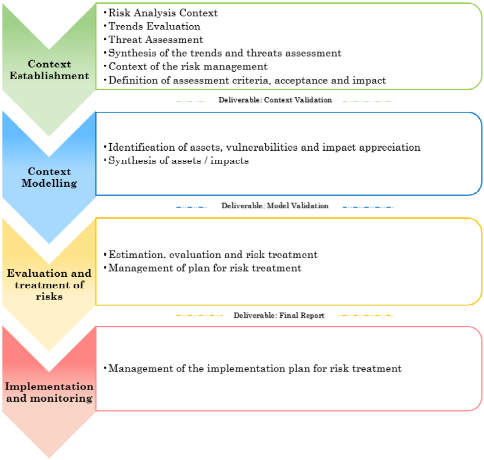
\includegraphics[scale=0.4]{./images/MONARC-method-2-1.png}
    \end{center}
\end{frame}

\begin{frame}
    \frametitle{ISO/IEC 27005:2011}
    \framesubtitle{Information risks}
    \begin{block}{Formula}
        $$R = I \times T \times V$$
        \begin{itemize}
            \item impact on \textbf{C}onfidentiality \textbf{I}ntegrity \textbf{A}vailability;
            \item on secondary assets.
        \end{itemize}
    \end{block}
\end{frame}


\begin{frame}
    \frametitle{ISO/IEC 27005:2011}
    \framesubtitle{Operational risks}
    \begin{block}{Formula}
        $$R = I \times P$$
        \begin{itemize}
            \item impact on ROLFP;
            \item on primary assets.
        \end{itemize}
    \end{block}
\end{frame}


\subsection{An optimized method}
\begin{frame}
    \frametitle{Optimizations}
    \framesubtitle{}
    MONARC is an optimized method:
    \begin{itemize}
        \item inheritance;
        \item scope of objects;
        \item models;
        \item deliverables.
    \end{itemize}
\end{frame}

\subsubsection{Inheritance}
\begin{frame}
    \frametitle{Inheritance}
    \framesubtitle{Modelling}
    \begin{center}
        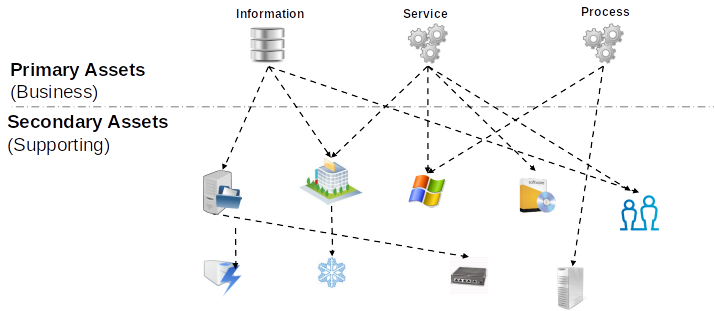
\includegraphics[scale=0.45]{./images/MONARC-method-modelling.png}
    \end{center}
\end{frame}

\begin{frame}
    \frametitle{Inheritance}
    \framesubtitle{Formalisation of the modelling}
    \begin{center}
        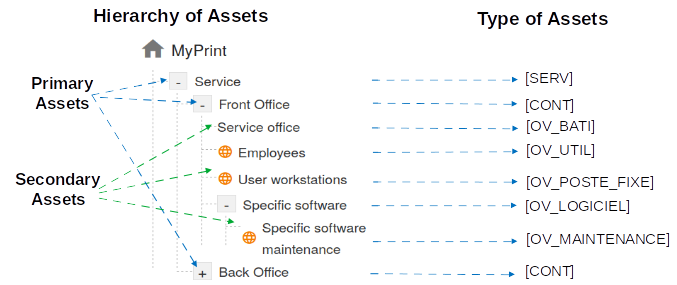
\includegraphics[scale=0.5]{./images/MONARC-modelling-formalisation.png}
    \end{center}
\end{frame}

\begin{frame}
    \frametitle{Inheritance}
    \framesubtitle{Formalisation of an asset}
    Example with \texttt{OV\_BATI}
    \begin{center}
        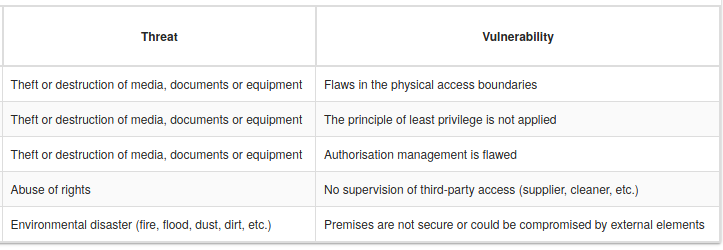
\includegraphics[scale=0.7]{./images/ov_bati.png}
    \end{center}
\end{frame}

\subsubsection{Scope of objects}
\begin{frame}
    \frametitle{Scope of objects}
    \framesubtitle{Global or local assets}
    \begin{center}
        \begin{center}
            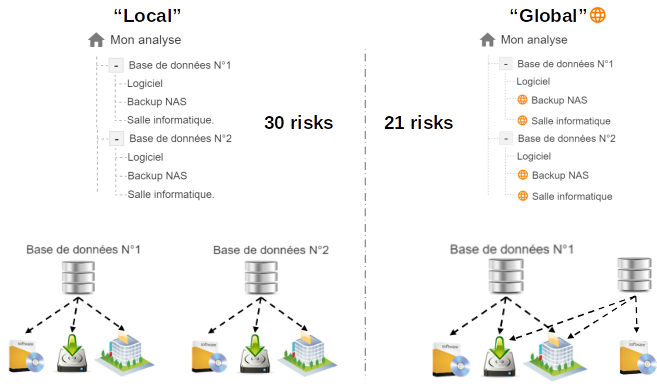
\includegraphics[scale=0.45]{./images/global-vs-local.png}
        \end{center}
    \end{center}
\end{frame}

\subsubsection{Inheritance}
\begin{frame}
    \frametitle{Inheritance of impacts}
    \framesubtitle{}
    \begin{center}
        \begin{center}
            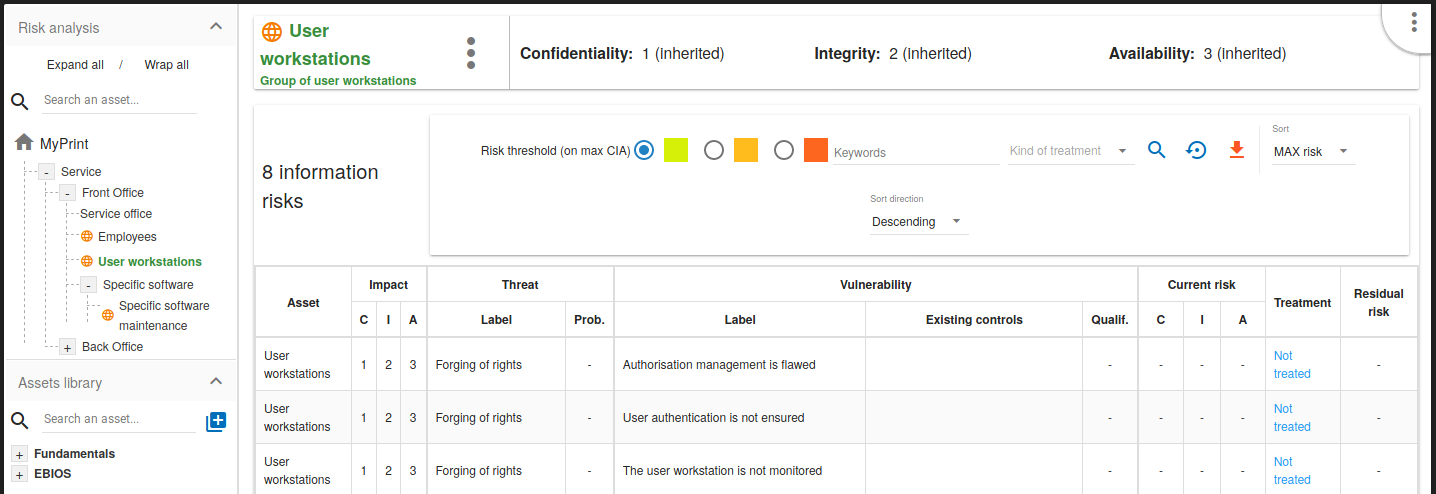
\includegraphics[width=12cm]{./images/impacts-inheritance.png}
        \end{center}
    \end{center}
\end{frame}

\subsubsection{Deliverables}
\begin{frame}
    \frametitle{Deliverables}
    \framesubtitle{}
    Shareable templates of deliverables.
\end{frame}
